% Presentation of Metajelo

\begin{frame}
  \frametitle{Reproducibility of research}

\begin{block}{Reproducibility and replicability of scientific findings has been given great scrutiny in recent years}

 \presencite{CamererEvaluatingreplicabilitylaboratory2016,Collaboration2015-ev,KleinInvestigatingVariationReplicability2014,FanelliOpinionsciencereally2018}.
\end{block}
\pause
\begin{block}{Historically, it has been difficult to find the materials required to conduct reproducibility or replication exercises}
	\presencite{Dewald1986,McCullough2006,McCullough03}.  
\end{block}
\end{frame}


\begin{frame}
\frametitle{Reproducibility of research}
\begin{block}{Journals are supporting the endeavor with ``Data [and Code] Availability Policies'' [DAP]}
	with variable success rates
	\presencite{stodden_enhancing_2016,stodden_toward_2013,Stoddenempiricalanalysisjournal2018,Hoeffler2017-tex}. 
\end{block}	

\pause
\begin{block}{Not a panacea}
	Despite DAPs, researchers often find that studies do not reproduce \presencite{Hoeffler2017a-tex,Chang2017,ChangLi2015,Stoddenempiricalanalysisjournal2018}
	
\end{block}

\end{frame}


\begin{frame}
\frametitle{Replication rates}
\begin{block}{Our own study}
% numbers from our study
% emphasize non-replication conditional on data
% then emphasize non-availability of data
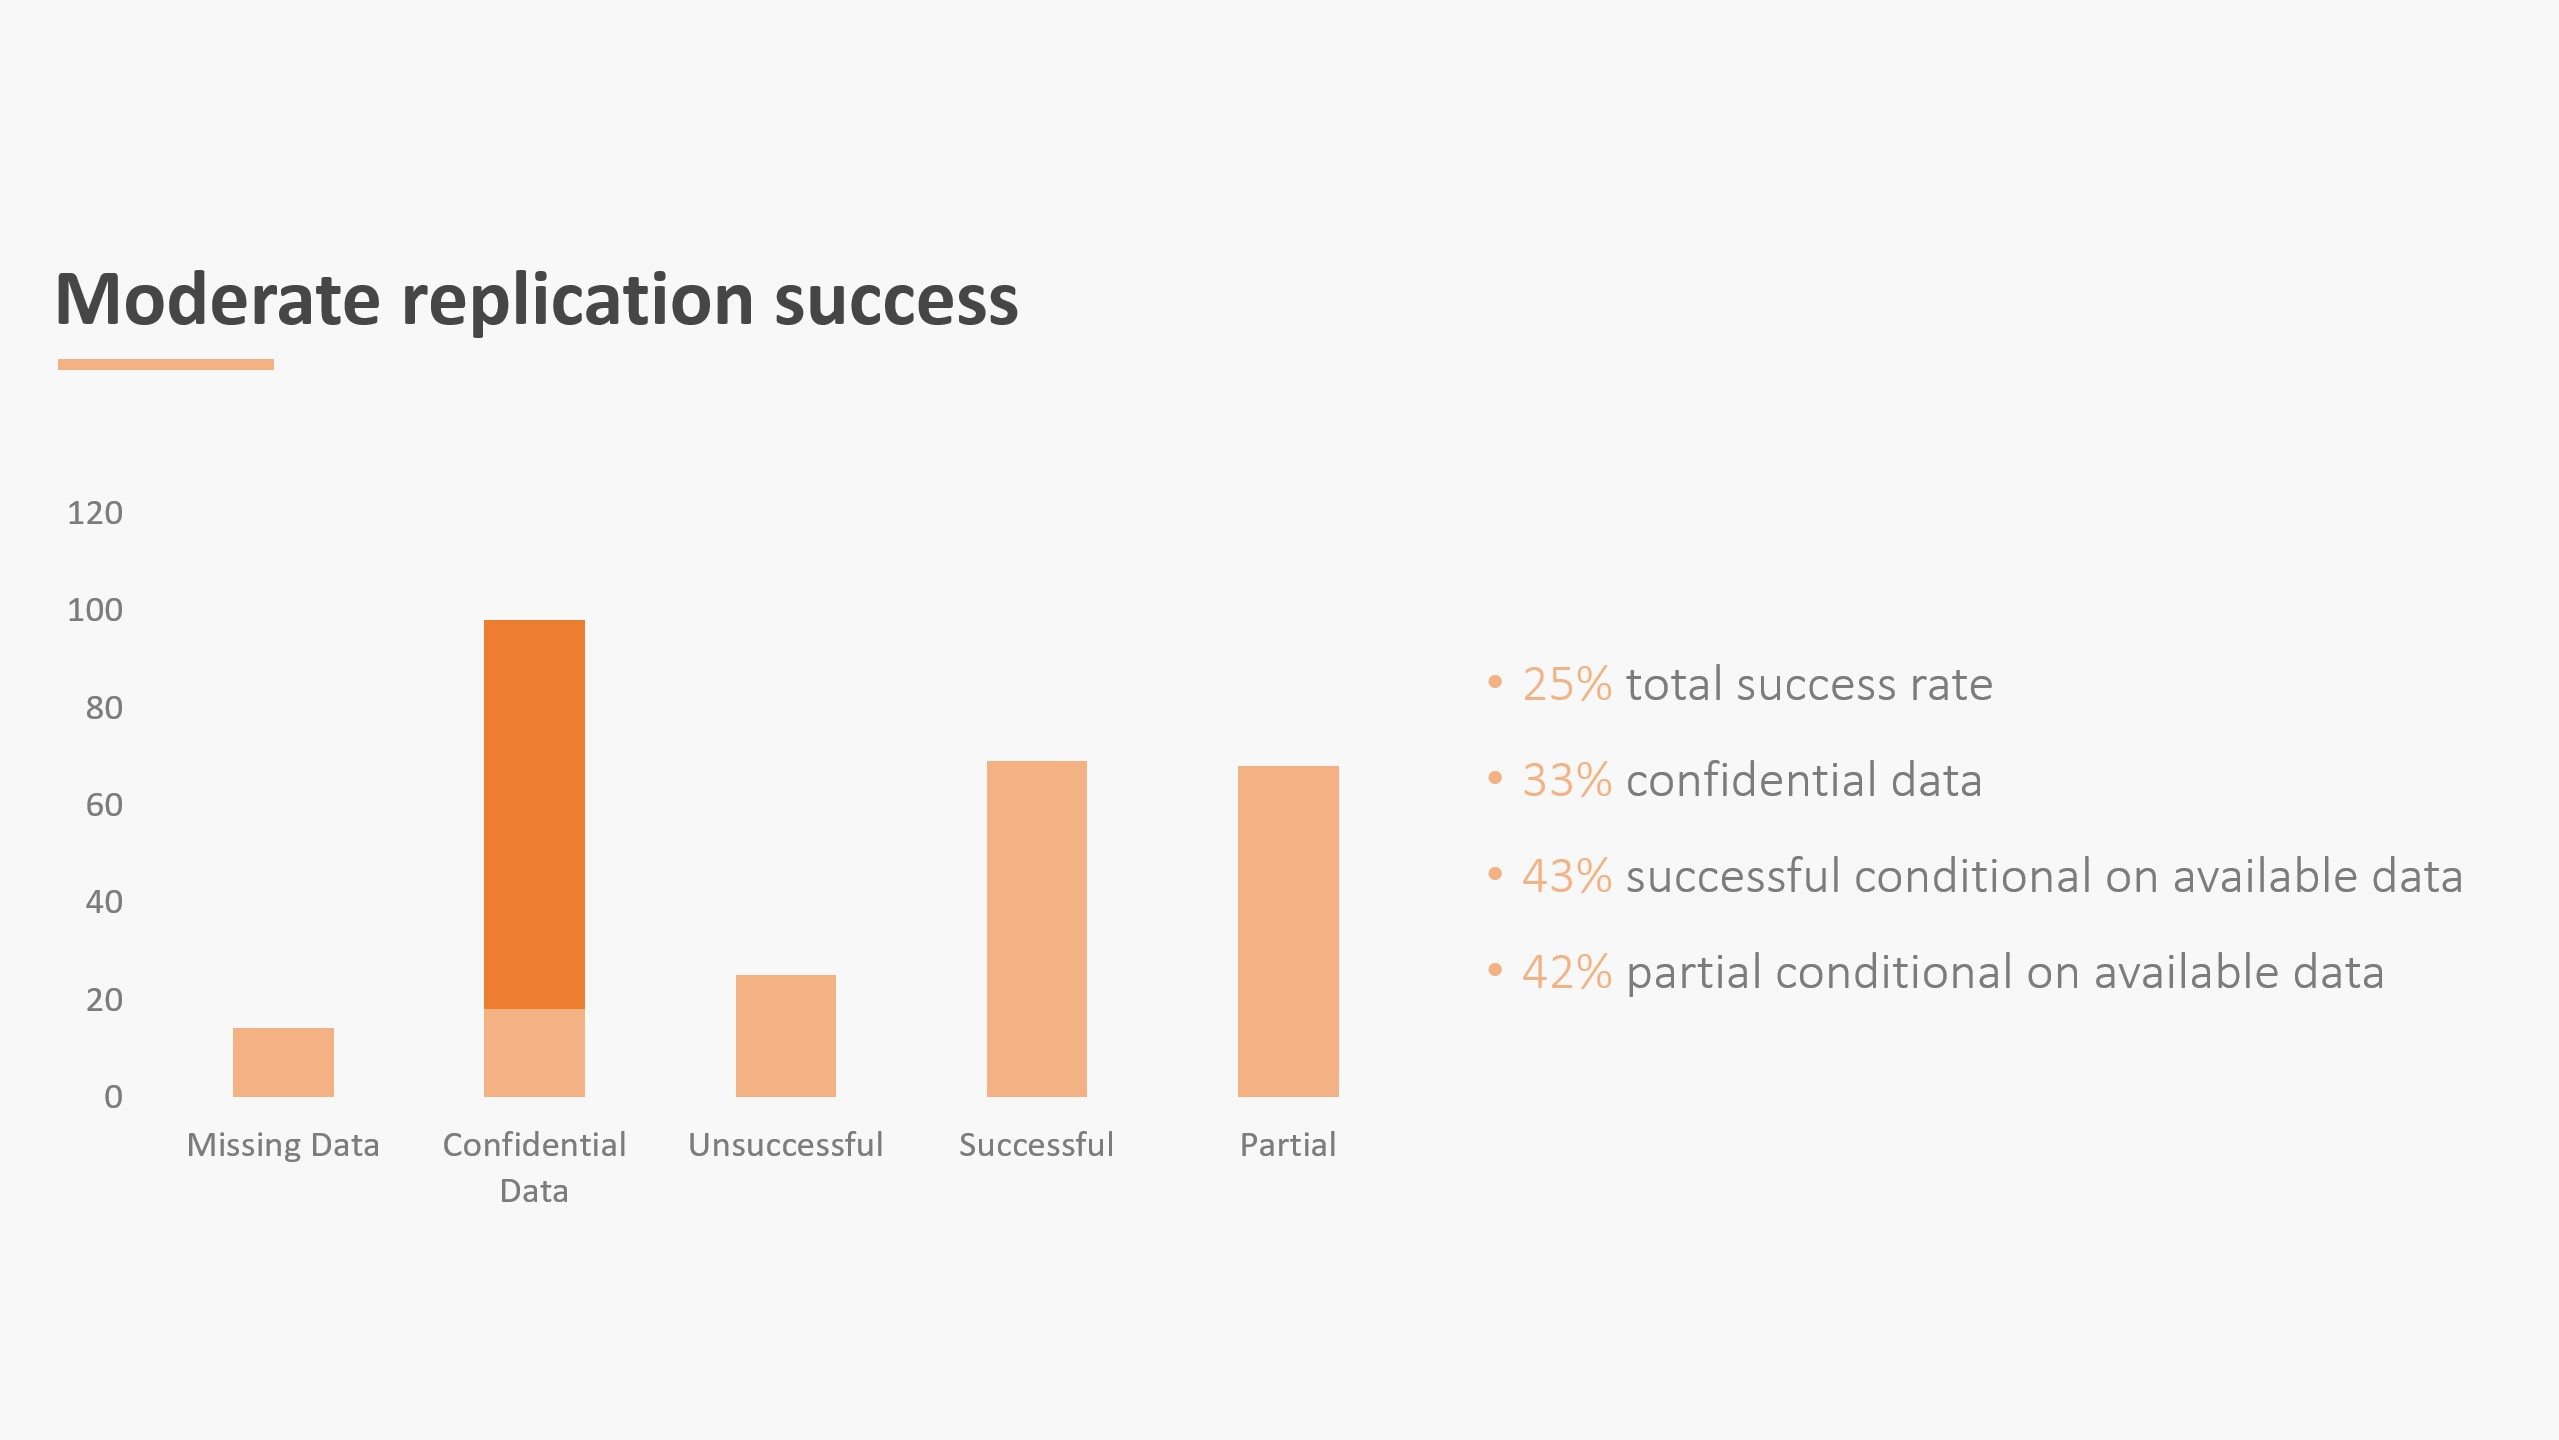
\includegraphics[width=0.9\textwidth]{images/bitss_slides_121018_Slide41.jpg}
\end{block}
\end{frame}


\begin{frame}
\frametitle{Restricted-access Data}
\begin{block}{Confidential Government Data}
	\begin{itemize}
		\item U.S. Census Bureau
		\item Statistisk sentralbyrå (Statistics Norway)
		\item many others
	\end{itemize}
\end{block}

\begin{block}{Confidential sub-national data}
	Just in the US:
	\begin{itemize}
		\item North Carolina Education Data
		\item Ohio Earnings and Education Statistics
		\item Oregon Health Data
		\item etc.
	\end{itemize}
\end{block}
\end{frame}

\begin{frame}
\frametitle{Restricted-access Data}
\begin{block}{Here in Australia}
Household, Income and Labour Dynamics in Australia (HILDA) Survey \textellipsis
\end{block}
\begin{center}
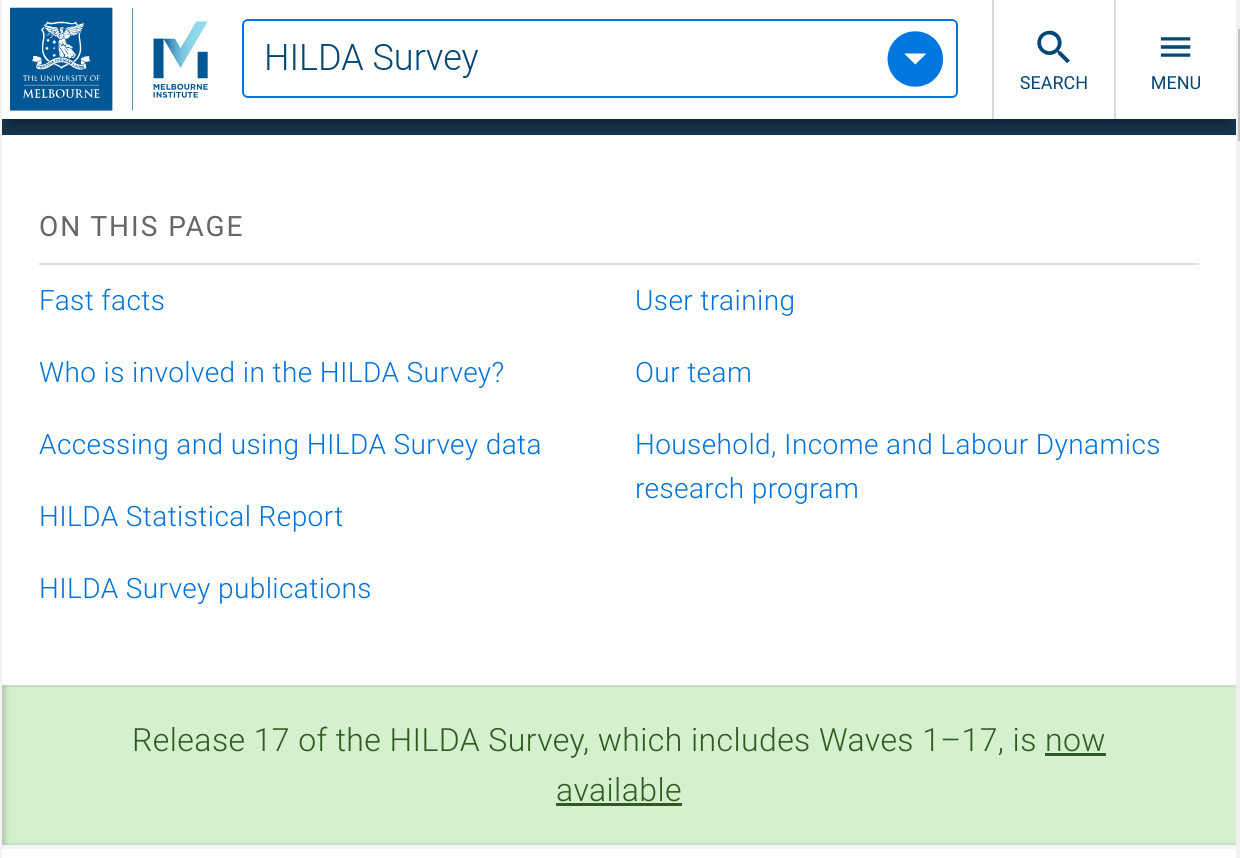
\includegraphics[width=0.95\textwidth]{images/hilda-screenshot1.png}
\end{center}
\end{frame}

\begin{frame}
\frametitle{Restricted-access Data}
\begin{block}{Here in Australia}
	Household, Income and Labour Dynamics in Australia (HILDA) Survey \textellipsis which is \textbf{restricted-access}
\end{block}
\begin{center}

\includegraphics[width=0.95\textwidth]{images/hilda-screenshot2.png}
		
\includegraphics[width=0.95\textwidth]{images/hilda-screenshot3.png}
\end{center}
\end{frame}



\begin{frame}
\frametitle{Restricted-access Data}
\begin{block}{Here in Australia}
	Household, Income and Labour Dynamics in Australia (HILDA) Survey \textellipsis which is \textbf{restricted-access}
\end{block}
\begin{center}
	
\includegraphics[width=0.95\textwidth]{images/hilda-screenshot4.png}
	
\includegraphics[width=0.95\textwidth]{images/hilda-screenshot5.png}
\end{center}
\end{frame}



\begin{frame}
\frametitle{Requirements for Reproducibility}
\begin{block}{What do we need?}
\begin{itemize}
	\item Description of the analysis (possibly as code)
	\item Access to the data
\end{itemize}
\end{block}
\end{frame}



\begin{frame}
\frametitle{Is restricted-access data compatible with reproducibility?}
\pause
\begin{block}{Answer: yes}
	\pause
\begin{itemize}
	\item Theoretical access to confidential  data: 
	\begin{itemize}
		\item More than \textbf{1000} users (not just Germans from Germany) have been granted access to German confidential labor market data  \presencite{Mueller2019} 
		\item More than \textbf{1500} users currently have access to confidential French data (\url{https://casd.edu})
		\item More than \textbf{700} researchers were active at the end of 2017 in the US Federal Statistical Research Data Centers (\href{https://www.census.gov/ces/pdf/2017_CES_Research_Report.pdf}{U.S. Census Bureau, 2018})
	\end{itemize}
\end{itemize}
\end{block}
\end{frame}

\begin{frame}
\frametitle{Is restricted-access data compatible with reproducibility?}
\pause
\begin{block}{Answer: yes}
\begin{itemize}
		\item Replications actually do occur with restricted-access data 
		\begin{itemize}
			\item[\ ]For instance, see exchange between \textcite{Godechot2016} and \textcite{CheminWasmer2017erratum} regarding \textcite{CheminWasmer2009},  using French (\href{https://quetelet.casd.eu/fr/utilisateur/connexion}{R\'eseau Quetelet}) data 
		\end{itemize}
	\end{itemize}
\end{block}
\end{frame}



\begin{frame}
\frametitle{Access Conditions}
\begin{block}{Is access \textbf{easy}?}
\begin{itemize}	\item No\end{itemize}
\end{block}\pause
\begin{block}{Is access \textbf{fast}?}
	\begin{itemize}	\item No\end{itemize}
\end{block}\pause
\begin{block}{Can \textbf{others} access the data?}
	\begin{itemize}	\item \textbf{Yes}!\end{itemize}
\end{block}
\begin{block}{Is there a \textbf{process} for granting access?}
	\begin{itemize}	\item \textbf{Yes}!\end{itemize}
\end{block}
\end{frame}





\begin{frame}
\begin{center}
\huge	No data, OK - surely we have  metadata on all those things?
\end{center}
\end{frame}


\begin{frame}
\begin{center}
	\huge	No.
\end{center}
\end{frame}



\begin{frame}
\frametitle{Lack of reliable metadata}
\begin{block}{\ }
	\large
 There is a 
 \begin{center}
 	\textbf{pervasive lack of consistent, reliable metadata} 
 \end{center}
on the materials provided to journals, and in particular those provided through third-party locations.
\end{block}
\end{frame}



\begin{frame}
\frametitle{Example 1: AEA journal}

\includegraphics[width=0.95\textwidth]{images/aeaweb-screenshot1.png}
\end{frame}

\begin{frame}
\frametitle{Example 1: AEA journal}

\includegraphics[width=0.95\textwidth]{images/aeaweb-screenshot2.png}
\end{frame}


\begin{frame}
\frametitle{Source code}
\lstinputlisting{aeaweb-current.xml}
\end{frame}

\begin{frame}
\frametitle{Example 1: AEA journal}
\begin{block}{AEJ: Applied Economics}
\begin{itemize}
	\item \textbf{Supplementary data} as ZIP file
	\item \textbf{Accessibility method}: download (obvious)
	\item \textbf{Accessibility conditions} or \textbf{license}: none stated (but in fact, {\color{red}Copyright with ``all rights reserved''}!)
	\item \textbf{Persistence}: assumed to be ``permanent'' because on journal website
\end{itemize}
\end{block}
\end{frame}



\begin{frame}
\frametitle{Example 2: Nature journal}
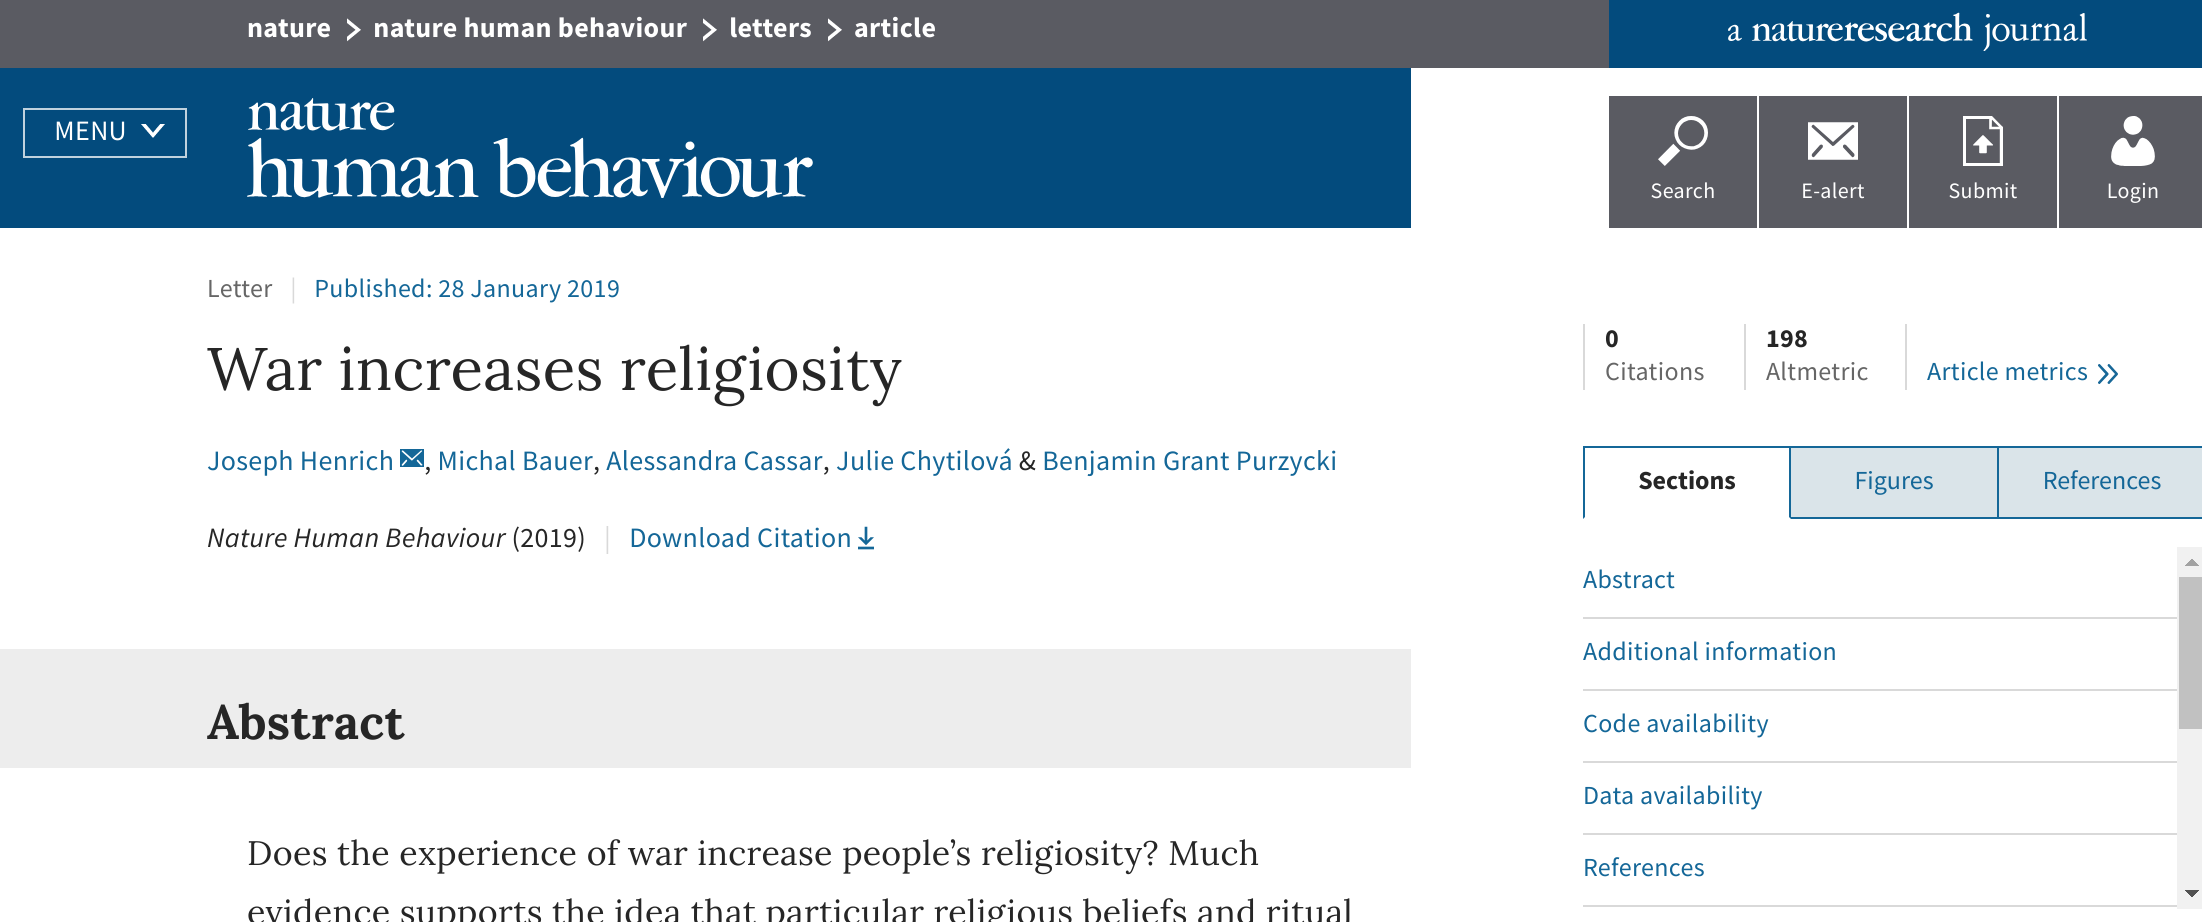
\includegraphics[width=0.95\textwidth]{images/nature-screenshot1.png}
\end{frame}

\begin{frame}
\frametitle{Example 2: Nature journal}
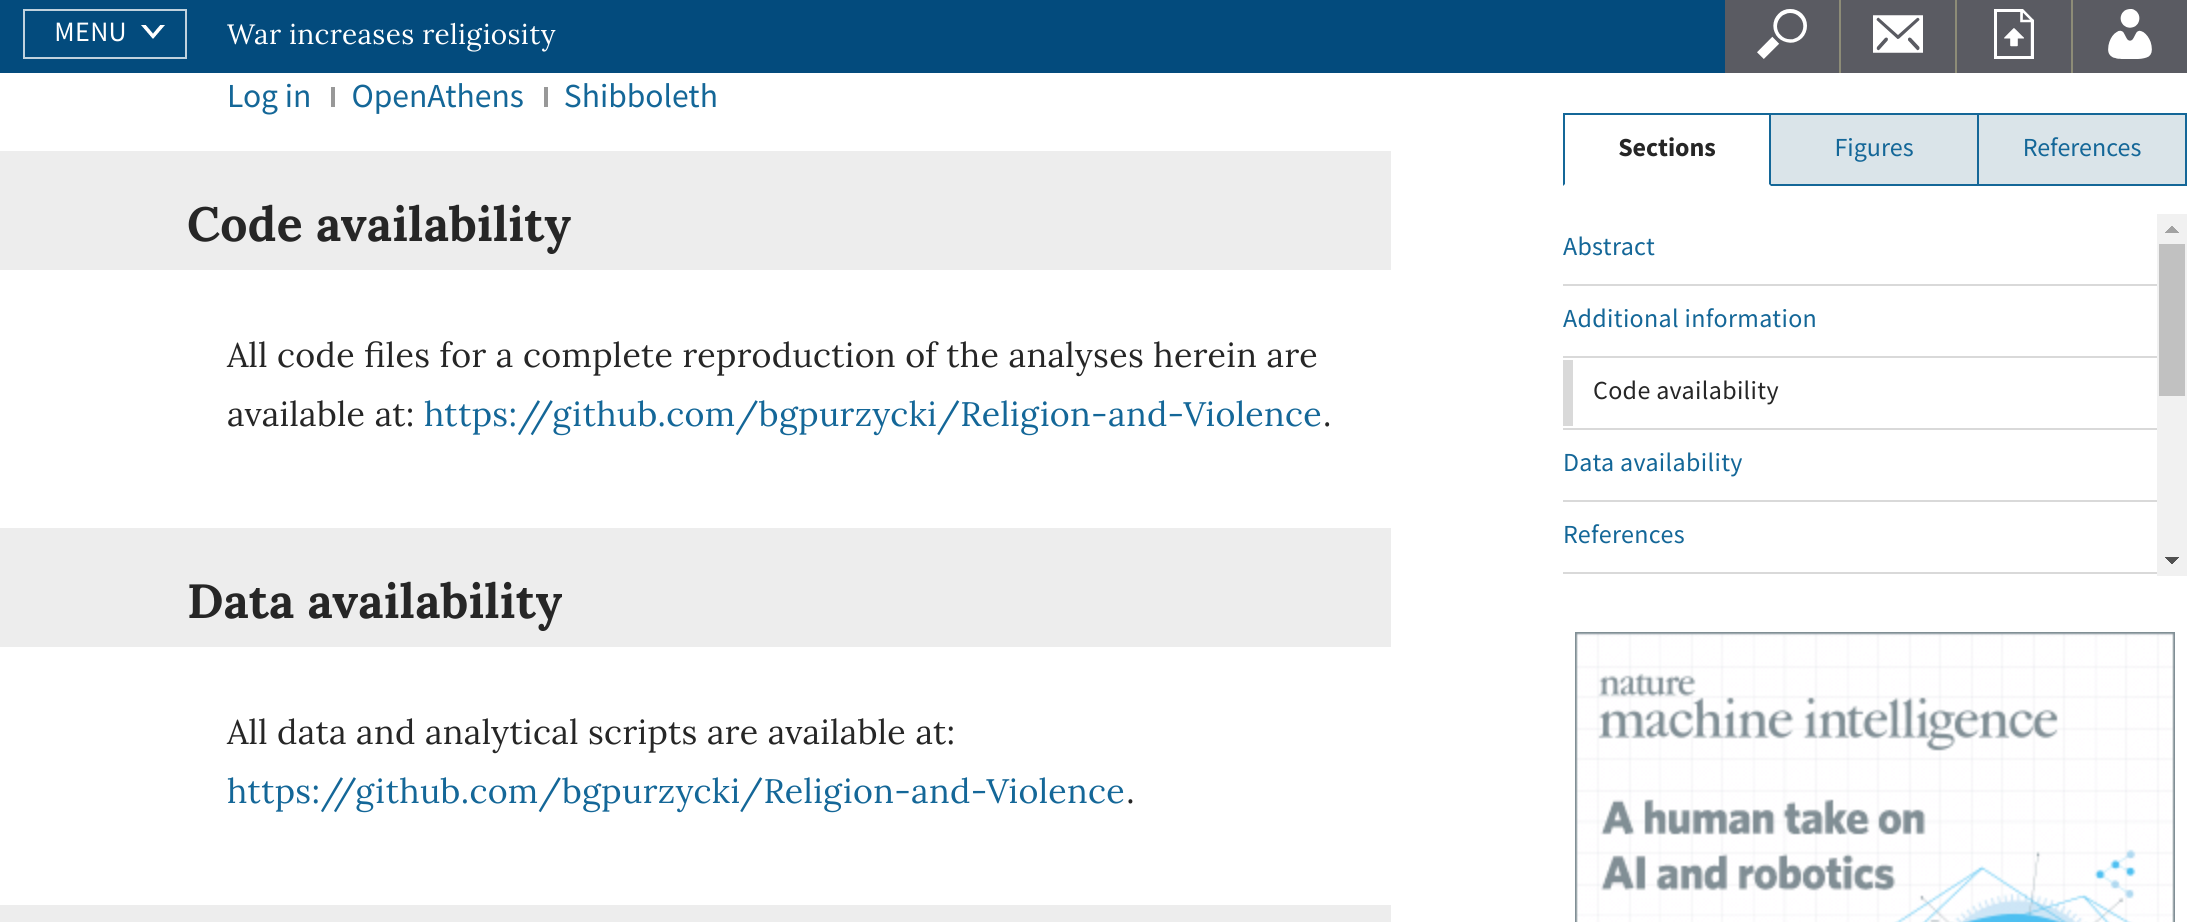
\includegraphics[width=0.95\textwidth]{images/nature-screenshot2.png}
\end{frame}


\begin{frame}
\frametitle{Source code}
\lstinputlisting{nature-current.xml}
\end{frame}

\begin{frame}
\frametitle{Example 2: Nature journal}
\begin{block}{Nature Human Behavior}
\begin{itemize}
\item \textbf{Supplementary data} as (manually!) linked Github archive
\item \textbf{Accessibility method}: unknown, but download presumed
\item \textbf{Accessibility conditions} or \textbf{license}: none stated on journal website, and in fact, none stated on Github site. Therefore: {\color{red}Copyright with ``all rights reserved''}!
\item \textbf{Persistence}: none stated, but use of Github is troublesome, as deletion is nearly instantaneous (at whim of author) and permanent 
\end{itemize}
\end{block}
\end{frame}


\begin{frame}
\frametitle{Current Metadata is Problematic}
\begin{block}{For \textbf{easily} accessible data}
	\begin{itemize}
		\item Unstructured
		\item Opaque
		\item Leads to imperfect, unreliable, failing replications
	\end{itemize}
\end{block}
\end{frame}


\begin{frame}
\frametitle{Current Metadata is Problematic}
\begin{block}{For \textbf{difficult to access} data}
	\begin{itemize}
		\item Highly unstructured (\textit{prose}) or inexistant
		\item Opaque
		\item Leads to imperfect, unreliable, failing replications
	\end{itemize}
\end{block}
\end{frame}



\begin{frame}
\begin{center}
	\huge Mission of journals: 
	
	Better transparency
\end{center}
\end{frame}



\begin{frame}
\begin{center}
	\huge \texttt{metajelo}
	
	\normalsize {\color{blue} metadata} (package) for 
	
	{\color{blue}journals}  to support 
	
	\color{blue} external 
	
	linked 
	
	objects
\end{center}
\end{frame}



\begin{frame}
\frametitle{Basic motivation}
\begin{block}{Publication-oriented}
	Provide journals with the metadata needed to assess the robustness and reliability of supporting materials.
	
\end{block}

\begin{block}{Minimal information}
Requests no more information than (in theory) is currently being requested from authors.
\begin{itemize}
	\item Name
	\item Location
	\item Accessibility (conditions, license)
	\item Persistence
\end{itemize}
\end{block}
\end{frame}


\begin{frame}
\frametitle{Basic motivation}
\begin{block}{Extensive re-use}
Leverage existing metadata \textit{\color{ForestGreen} schemas} and \textit{\color{MidnightBlue} infrastructure} as much as possible
\begin{itemize}
	\item Re-use of {\color{ForestGreen} DataCite} and {\color{ForestGreen} re3data} metadata elements
	\item Overlapping elements map into Dublin Core, CrossRef, DDI
\end{itemize}
\end{block}
\end{frame}



\begin{frame}
\frametitle{Structure of \texttt{metajelo}}
\begin{block}{Each package is a linkage record}
	\begin{itemize}
		\item  conceptually models a linkage between a publication and its supplementary materials
		\item A record has an \textbf{identity} (\ac{DOI}), a \textbf{date created}, a \textbf{last modified date}, and the \textbf{identity} (\ac{DOI}) \textbf{of the research objects} (papers) that are associated with the supplementary products
		\item Then an unlimited number of \texttt{supplementaryProducts}
	\end{itemize}
\end{block}
\end{frame}
		
\begin{frame}
\frametitle{Structure of \texttt{metajelo}}
\begin{block}{Each \texttt{supplementaryProducts} has}
	\begin{itemize}
	\item  an identifier, 
	\item a description of its \textbf{type}, 
	\item linkages to full metadata available elsewhere that fully describes the product.  
	\item an associated location block (institutional archive)
	\item the set of possible policies (\textbf{access, license, preservation}), with a boolean designation flagging the relevant policy for the particular object
	\item Each policy instance structured to allow for verbatim answers if necessary
\end{itemize}
\end{block}
\end{frame}



\begin{frame}
\frametitle{Detailed Structure}
\begin{block}{Full annotated schema}
	
\href{https://github.com/labordynamicsinstitute/metajelo}{github.com/labordynamicsinstitute/metajelo}
\end{block}
\end{frame}



\begin{frame}
\huge About that \textit{\color{MidnightBlue} infrastructure} \textellipsis
\end{frame}


\begin{frame}
\frametitle{Shortcoming of existing metadata}
\begin{block}{Why not directly collect the information from \textit{\color{MidnightBlue} infrastructure}}
	
\end{block}
\end{frame}

\begin{frame}
\frametitle{Much information lacking from current infrastructure}
Paper goes into detail about the \textbf{failures of the current infrastructure} to provide information even when the objects are registered by knowledgeable institutions, and despite the ability to do so \textbf{within existing metadata schemas}.
\end{frame}



\begin{frame}
\frametitle{How to generate a \metajelo package?}
\begin{block}{Enable authors}
 Develop an application to allow users to generate a \metajelo package
 \begin{itemize}
 	\item Leveraging infrastructure where possible
 	\item Querying the user where necessary
 \end{itemize}
\end{block}
\begin{block}{Portability}
	Once created, a \metajelo package should be of use at multiple journals: saved locally
\end{block}
\end{frame}

\begin{frame}
\frametitle{How to generate a \metajelo package?}
\begin{block}{Encourage data providers}
	All information can be provided by data providers in a static format
	\begin{itemize}
		\item Generate once, deposit on website
		\item (optional) leverage to display suggested data citations
	\end{itemize}
\end{block}
\end{frame}


\begin{frame}
\frametitle{How to \textbf{use} a \metajelo package?}
\begin{block}{Enable journals}
	The information should be leverable with minimal modifications to current journal infrastructure
	\begin{itemize}
		\item Simplest: attach \metajelo package, leverage CSS and JS to display contents
		\item More robust: ingest in journal management system
	\end{itemize}
Short-term implementation can be made, without preventing future robust implementation
\end{block}
\end{frame}

\begin{frame}
\frametitle{Sketch of a user-facing app}
\begin{tabular}{cc}
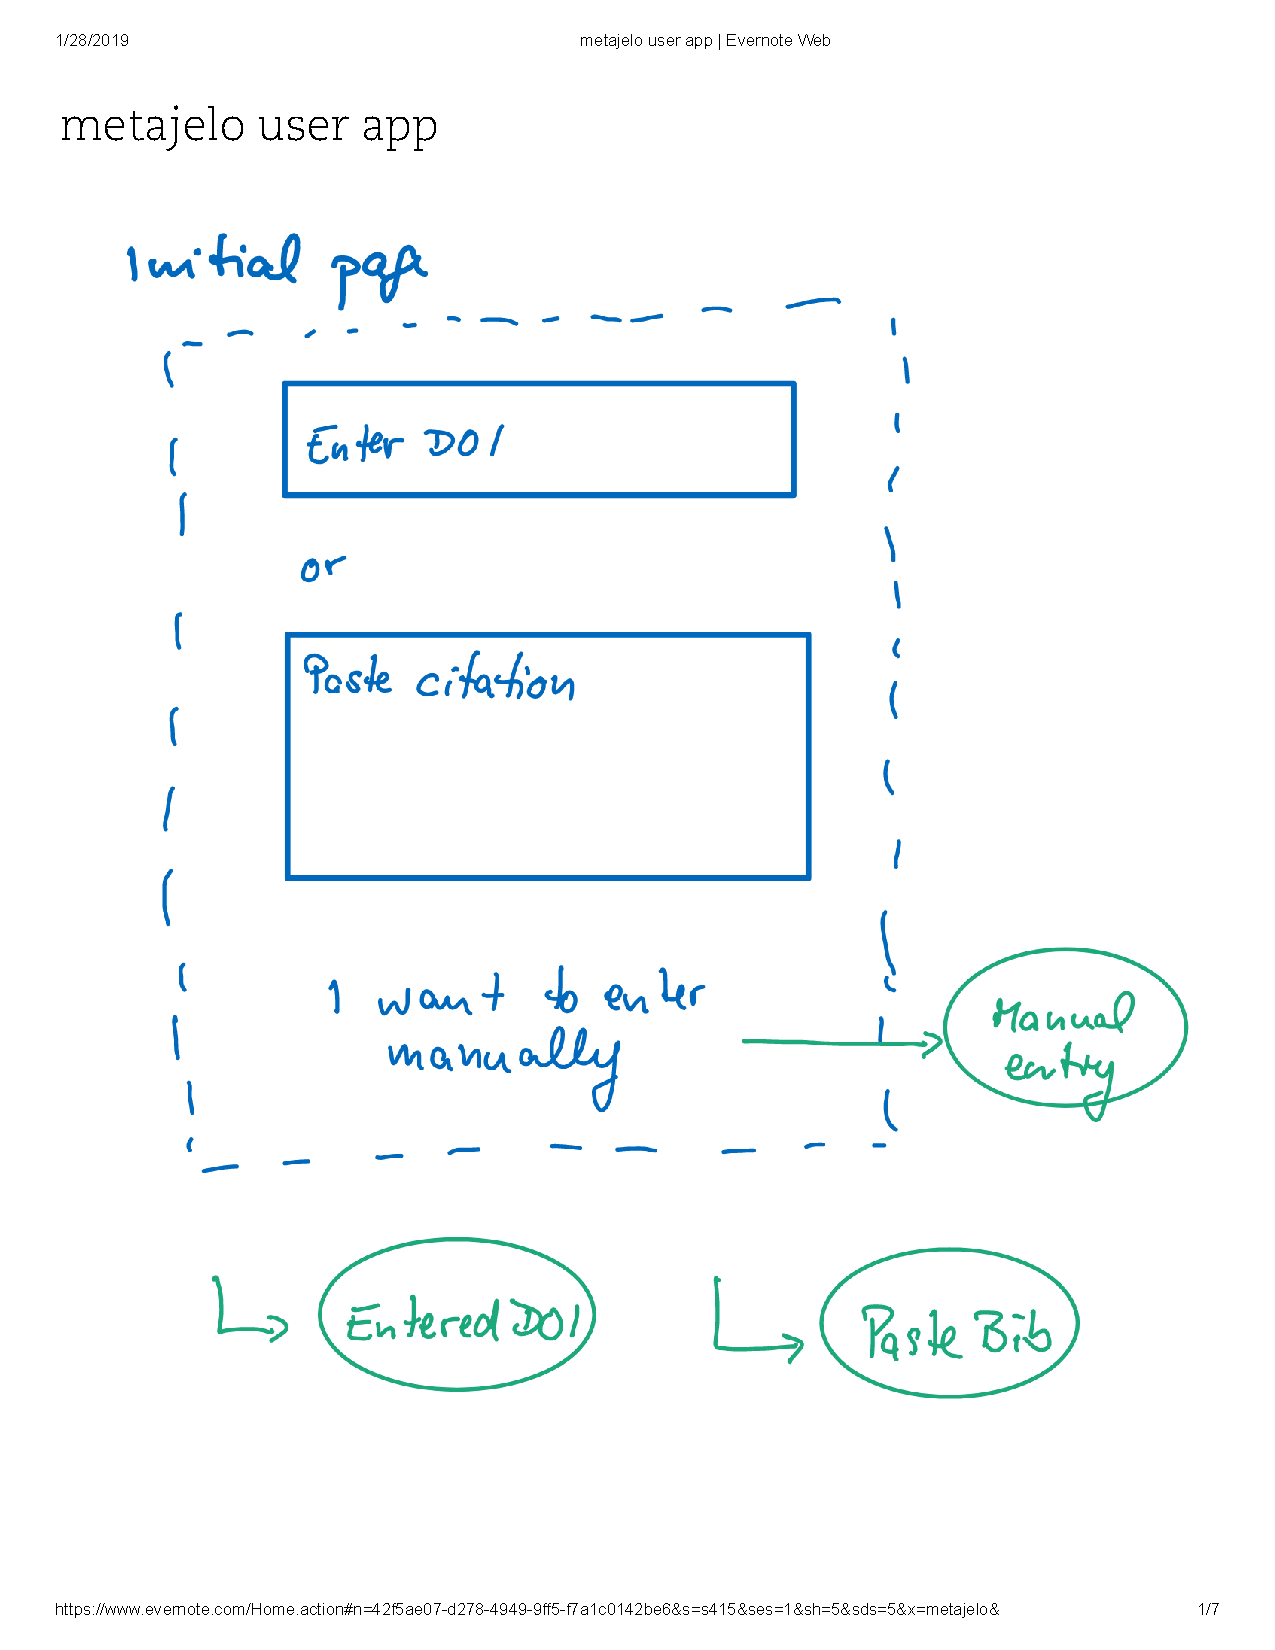
\includegraphics[page={1},height=0.7\paperheight]{images/metajelo-user-app-Evernote.pdf}
&
\includegraphics[page={7},height=0.7\paperheight]{images/metajelo-user-app-Evernote.pdf}
\end{tabular}
\end{frame}

\begin{frame}
\frametitle{Sketch of a website}
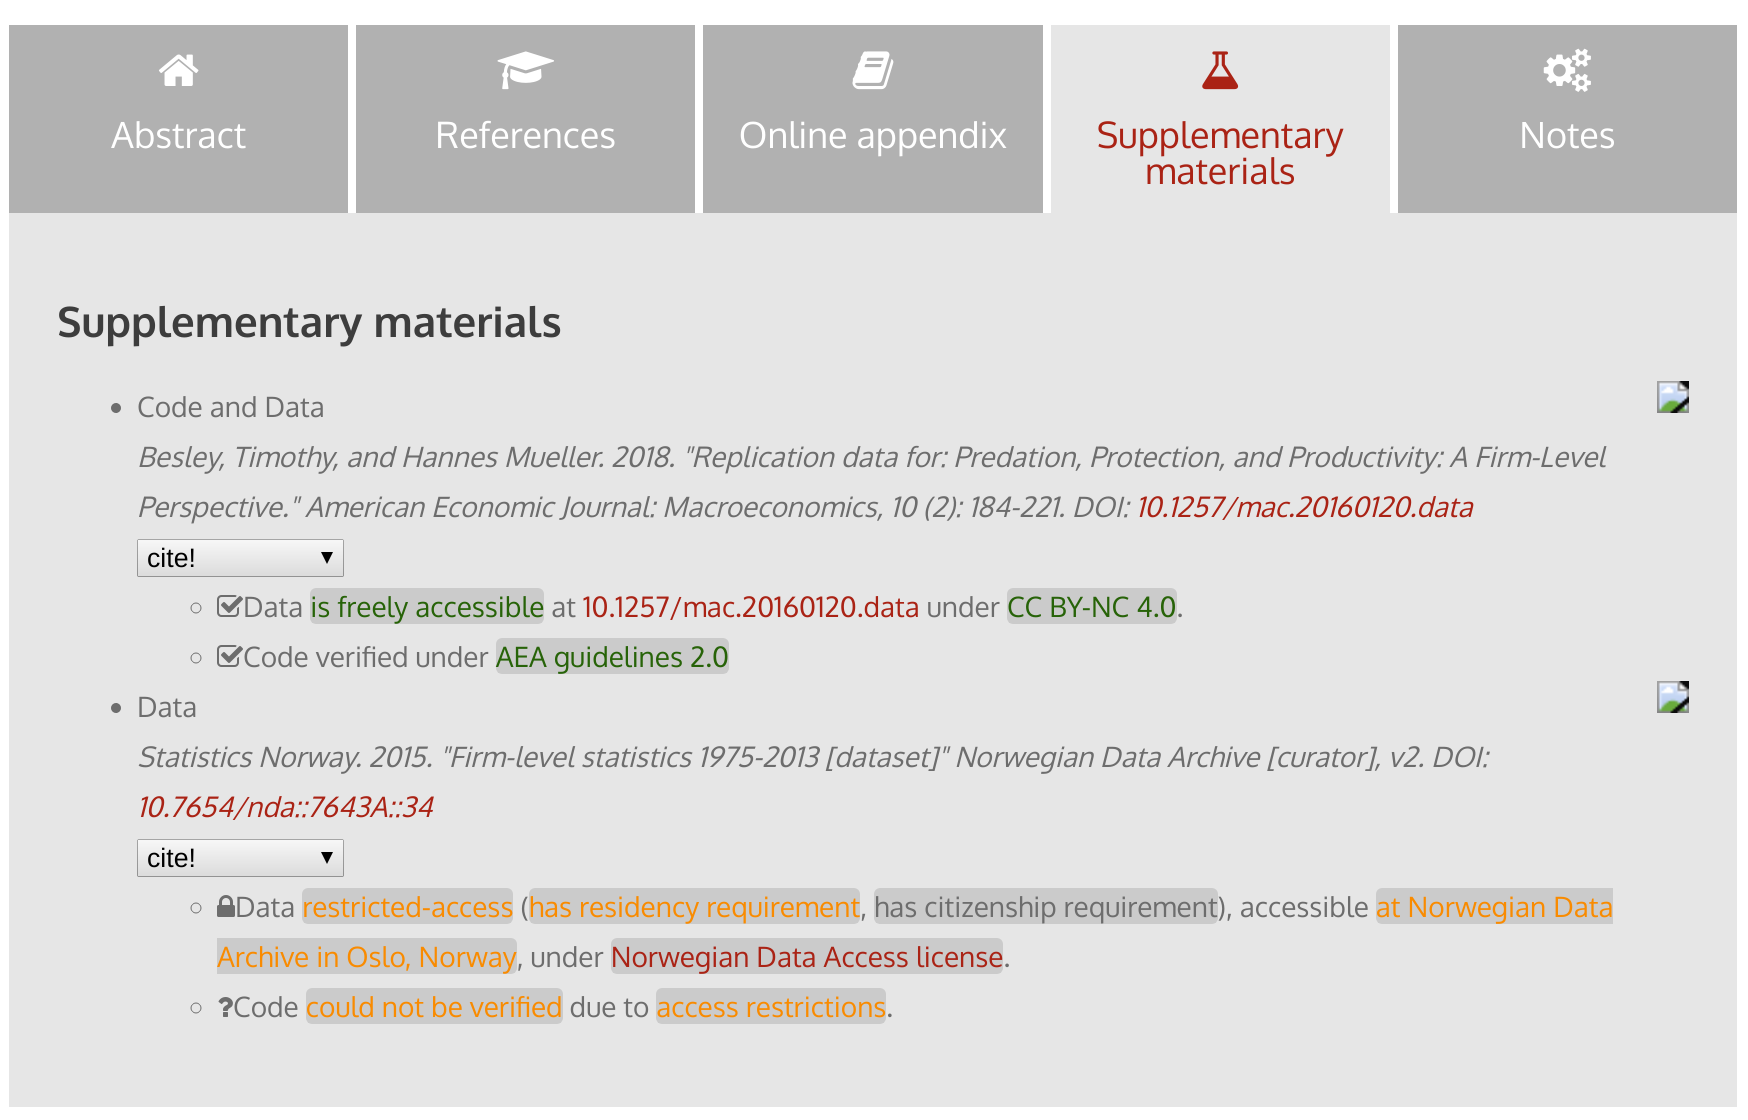
\includegraphics[height=0.7\paperheight]{images/aeaweb-demo1.png}
\end{frame}

\begin{frame}
\frametitle{Sketch of a website}
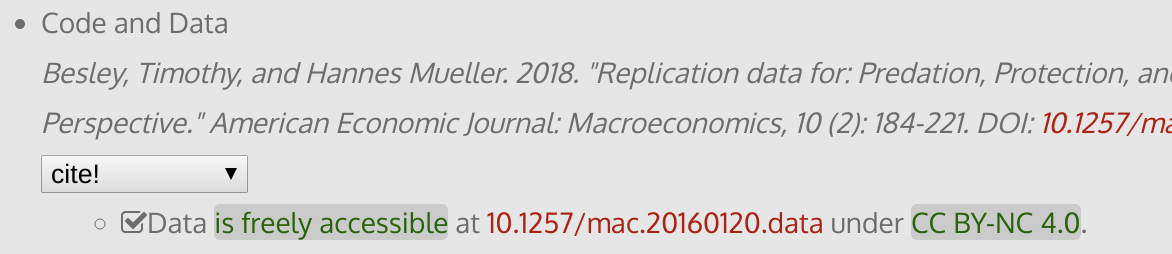
\includegraphics[width=0.8\paperwidth]{images/aeaweb-demo2.png}
\end{frame}



\begin{frame}
\frametitle{Next steps}
\begin{block}{Community input}
	We want to hear from a broad community about utility, extensions, etc.
\end{block}
\begin{block}{Development of apps}
	We have started development of both \textbf{user-facing apps} and \textbf{journal-oriented toolkit}
\end{block}
\begin{block}{Implementation}
	This is part of a broader strategy to improve transparency and reproducibility at the American Economic Association and in economics in general
\end{block}
\end{frame}


\begin{frame}
\centering \Huge Thank you
\end{frame}
